%%% template.tex
%%%
%%% This LaTeX source document can be used as the basis for your technical
%%% paper or abstract. Intentionally stripped of annotation, the parameters
%%% and commands should be adjusted for your particular paper - title, 
%%% author, article DOI, etc.
%%% The accompanying ``template.annotated.tex'' provides copious annotation
%%% for the commands and parameters found in the source document. (The code
%%% is identical in ``template.tex'' and ``template.annotated.tex.'')

\documentclass[conference]{acmsiggraph}

\usepackage{authblk}
\usepackage[]{algorithm2e}

\TOGonlineid{45678}
\TOGvolume{0}
\TOGnumber{0}
\TOGarticleDOI{1111111.2222222}
\TOGprojectURL{}
\TOGvideoURL{}
\TOGdataURL{}
\TOGcodeURL{}

\title{Performance Driven Redundancy Optimization of Data Layouts for Walkthrough Applications}

%\author[1]{Zachary DeStefano\thanks{zdestefa@uci.edu}}
%\author[1]{Shan Jiang\thanks{sjiang1714@gmail.com}}
%\author[1]{Gopi Meenakshisundaram\thanks{gopi.meenakshisundaram@gmail.com}}
%\author[2]{Sung-Eui Yoon\thanks{toinsert}}
%\pdfauthor{Zachary DeStefano,Shan Jiang,Gopi Meenakshisundaram,Sung-Eui Yoon}
\pdfauthor{}
\author{}
%\affil[1]{University of California, Irvine}
%\affil[2]{KAIST}

\keywords{Data Layout Problem, Out-Of-Core Rendering, Cache Oblivious Mesh Layout, Redundant Data Layout, Walkthrough Application}

\begin{document}

%% \teaser{
%%   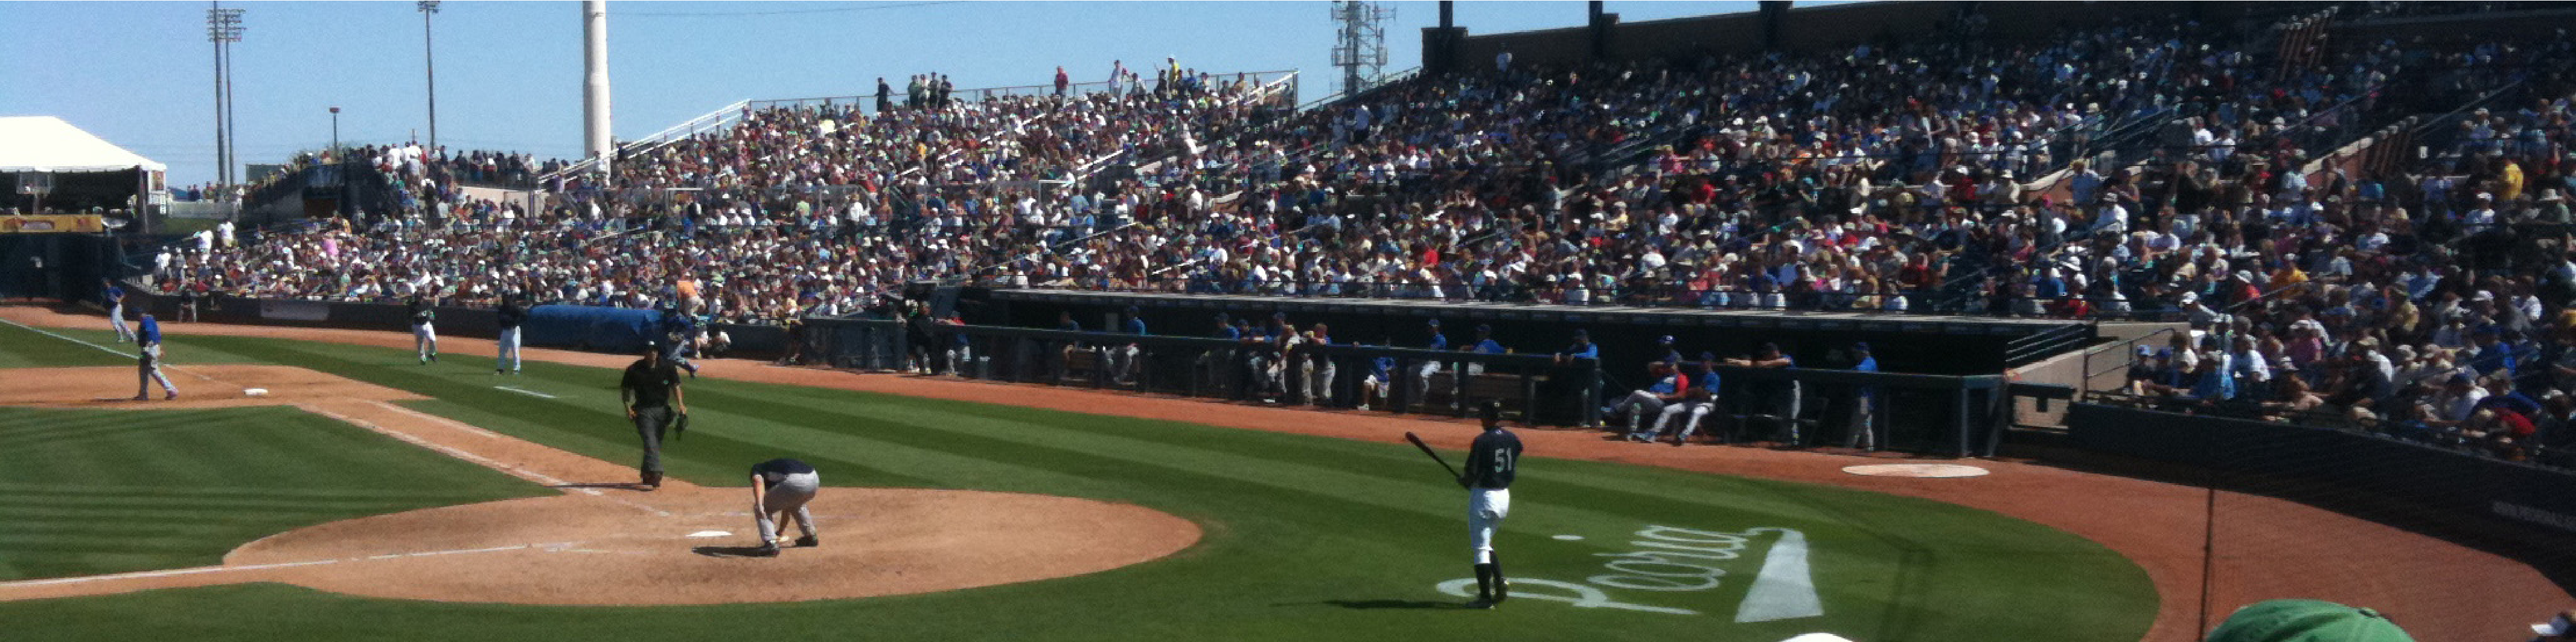
\includegraphics[height=1.5in]{images/sampleteaser}
%%   \caption{Spring Training 2009, Peoria, AZ.}
%% }

\maketitle

\section{Run-time and Storage Analysis}

We now analyze the running time and storage requirements of our algorithm. We will denote $N$ as the number of data units and $A$ as the number of access requirements. We will use $k$ as the average span of a single access requirement. The variable $Q$ will represent how many executions of the redundancy loop occur. The average number of overlapping access requirements is proportional to the number of data units multiplied by the redundancy factor $r$, which is the amount of redundancy if we have a single-seek layout. Therefore, the number of overlapping access requirements is $O(rN)$. 

\subsection{Run-time Analysis}

The loop that initially constructs the access requirement heap is run on all $A$ access requirements. It involves finding all the benefit information and putting it into a heap so that it is easy to figure out the best access requirement to modify first. With each run of the loop, in addition to a constant number of initial operations, there are $log(A)$ operations to insert the data into the heap plus $O(k)$ operations for the search of the AR to get the benefit information. Thus it takes a total of $O(A (k + logA))$ operations to do the initial construction. \\
\\
With the following loop which actually copies the data units and updates the information, there are a total of $Q$ executions of it. In addition to the constant number of operations, each execution of the loop has to go through each of the overlapping access requirements and update their data. There are $O(rN)$ overlapping access requirements. For each of the affected access requirements, there are $O(k + log(A))$ operations to recalculate the benefit data and reform the heap. Thus the final loop takes $O(QrN(k + logA))$ operations. \\
\\
This means that in total, our algorithm takes $O((QrN + A)(k + logA))$ operations. In all likelihood, we will have to run the loop at least once, so $Q \geq 1$. Additionally, since $r \geq 1$, we know that $rN \geq A$. Thus we can simplify the expression to say that our algorithm takes $O(QrN(k + logA))$ operations. Because we only have polynomial or logarithmic terms, we have found an algorithm that is efficient given our input size for computing an optimized layout.

\subsection{Storage Analysis}

During the run of the algorithm, we have to store the number of overlapping access requirements at each data unit, which will require $O(N)$ storage. We will also have to store a heap of access requirements, which can be stored using $O(A)$ space. We also have a list of access requirements and that information will take up $O(A)$ space. In total we thus have $O(A + N)$ storage space used during the run of the algorithm. 


\subsection{Linear search justification}

Here I justify why we do a simple element by element search on the set of possible data units in the part of the algorithm where we decide where to put the copy. The original problem is to find the least number in an arbitrary block of a list. This is because each data unit stores the number of overlapping access requirements so we have a list of numbers to search through. There are only a limited number of data units where we could move the copy to hence we only care about an arbitrary part of this list. If $k$ is the size of the access requirement, then the searching gives us $O(k)$ query time. Updates will also be $O(k)$ and construction will be $O(N)$ with N being the number of data units. There are other approaches, such as a range tree or dynamic programming, that may produce better query times, but their construction and update times will be worse as well as their storage. \\
\\
With dynamic programming, we would have to maintain a matrix where an entry $(i,j)$ would contain the minimum value in that range. This would give us a $O(1)$ query time but the construction and storage would be $O(N^2)$ where N is the number of data units. The update time would be $O(N)$ when we add a data unit. Since the $N$ for this problem domain is in the hundreds of millions, that is an unacceptable storage bound. The construction run time would also be prohibitive given the magnitude of our input. \\
\\
We could use a range tree. The initial binary search tree would be sorted by index and at each entry would be a pointer to a binary search tree sorted by value. If we put the min value at each of the nodes of the initial tree, we can speed up our queries. We would get a $O(log N)$ query time, but our construction time and storage would be $O(N log N)$. Updating the data structure would take at a minimum $O(k log(N))$ time if we do careful indexing and only update the nodes that need to be updated. If we have a large access requirement, then this would represent a significant improvement in query time however given our exceptionally large input, the construction, storage, and update bounds are too prohibitive.  


In the algorithm, we make a list of data units that will reduce seek time by just moving them. We perform these moves first before doing any copying. This initial step will produce a better solution than proposed by \cite{cacheobliviouslayout} without adding extra units. This is because our algorithm will consider cases where data units are close to each other but in hierarchically different blocks with  the cache oblivious layout. To show this, consider a case where we have two access requirements of 5 data units each. Figure \ref{YoonImprovement} shows an example of that kind of layout. In the middle of that figure is the result of using the cache oblivious layout. Because hierarchically it would arrange the units in each block and then arrange the blocks, it does not detect that the units with the black access requirement can be grouped together. When our algorithm is run, it would find that it can shorten the black access requirements without adding redundancy so it would do that first, as shown in the bottom of that figure.

\begin{figure}[ht]
\centering
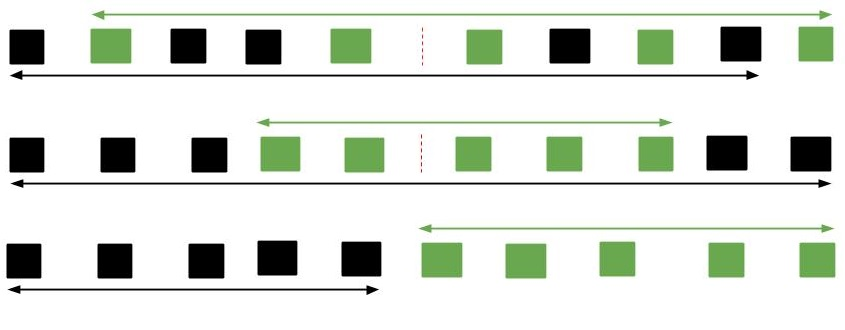
\includegraphics[width=3in]{ImprovementOverYoon.jpg}
\caption{Example of two access requirements of 5 data units each. The red line represents the boundary between blocks in the cache oblivious layout hierarchy. The original layout (top), cache-oblvious layout (middle), as well as the layout after running our algorithm (bottom) is shown.}
\label{YoonImprovement}
\end{figure}

Existing algorithms for the data layout problem do not consider redundancy. Even if we find a polynomial time algorithm that solves the data layout problem, we can actually achieve a seek time better than the optimal one without redundancy. We have such an example with figure \ref{fig:startingProb}. As can be seen in the figure, the total seek time is 11 units originally. Without redundancy, the seek time is reduced to 9 units, as found through a brute-force search. With redundancy, the total seek time is the minimum required which is 8 units. While a reduction from 9 to 8 units may not seem dramatic, when this result is scaled up to the hundreds of millions, this makes a big difference in seek time, which we saw in practice.\\

\begin{figure}[ht]
\centering
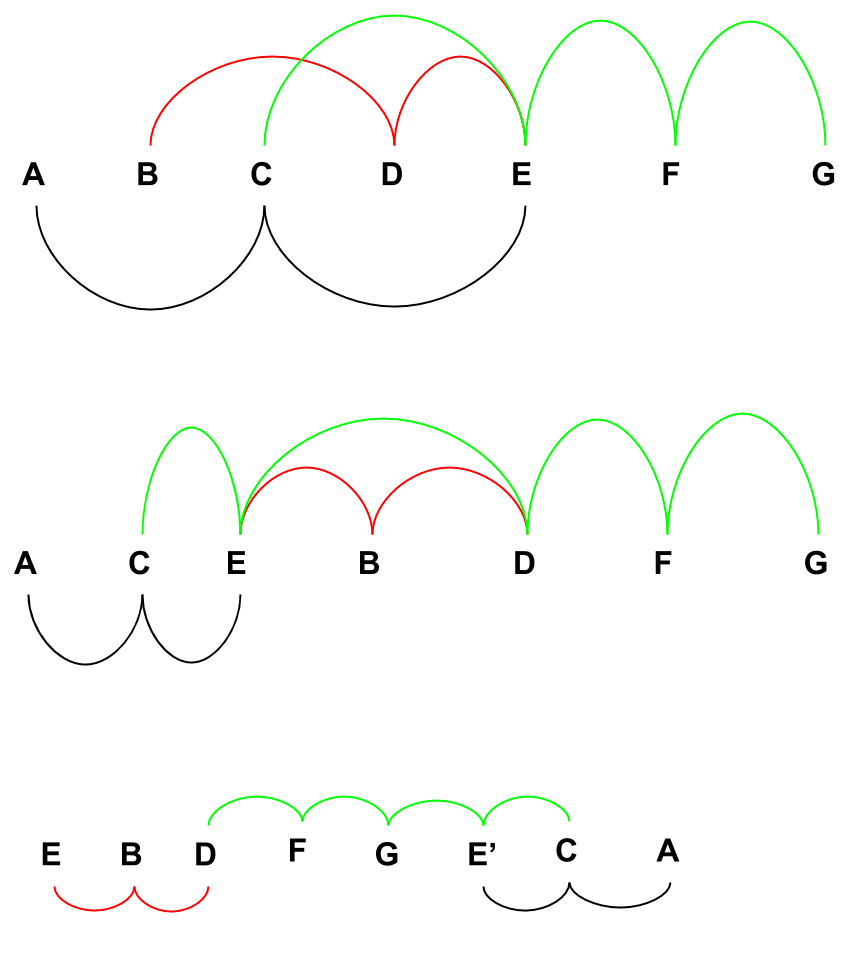
\includegraphics[width=3in]{examplePic.png}
\caption{Data Units with varying access requirements (top) as well as its optimal layout without redundancy (middle) and its optimal layout with redundancy (bottom)}
\label{fig:startingProb}
\end{figure}

\bibliographystyle{acmsiggraph}
\bibliography{finalPaperRefs}

\end{document}
